\documentclass[12pt]{article}
\usepackage[utf8]{inputenc}
\usepackage{graphicx}
\usepackage{amsmath}
\usepackage{geometry}
\usepackage{hyperref}
\geometry{margin=1in}

\title{Financial Data Engineering Pipeline}
\author{Nestor Torrech}
\date{\today}

\newcommand{\imgpath}{C:/Career Projects/Index Predictions/Outputs/Images}

\begin{document}

\maketitle

\begin{abstract}
This report documents the design and implementation of a Python-based data engineering pipeline for ingesting, processing, visualizing, and storing financial time series data. The pipeline collects data from the Tiingo API, transforms it into monthly and weekly summaries with engineered features such as returns and volatility, visualizes trends over time, and then uploads the data to a PostgreSQL database.
\end{abstract}

\section{Introduction}
In recent times, Index Fund Investing has grown as a popular alternative to picking individual stocks. Through this method, investors can keep their holdings in a single asset that represents multiple companies across various industries in both US Markets and abroad. The goal of this project is to automate the collection and processing of financial data to look at a selection of Index Funds. The pipeline computes derived metrics such as 30-day and 7-day moving averages and volatility, visualizes performance over time, and stores results in a structured SQL database for downstream analysis.

\section{System Architecture}
The pipeline consists of three main components:
\begin{enumerate}
\item \textbf{Data Cleaning:} Reads and processes raw time series data.
\item \textbf{Graphs:} Generates visualizations to explore trends.
\item \textbf{SQL Upload:} Uploads cleaned and deduplicated data to PostgreSQL.
\end{enumerate}

\section{Data Cleaning (01.00.Data\_Cleaning.ipynb)}
This script downloads historical daily prices for a list of tickers from the Tiingo API. It then applies the relevant data transformations to make the data useful for the analyst.

\subsection{Monthly}
The monthly transformation process begins by sorting the long-format time series data by both ticker and date to ensure calculations follow chronological order. The script computes the daily return as a percentage change from the previous day's closing price, which offers a basic measure of short-term price movement. Next, it calculates a 30-day moving average of the closing price, which smooths out daily fluctuations and highlights longer-term trends for each security. Additionally, the script computes intraday volatility, defined as the percentage difference between the open and close price on a given day. These metrics—return, moving average, and volatility—are all calculated within each ticker's group.

To enable aggregation at a monthly level, the script creates a new column that extracts the month and year from the date column. It then groups the data by both Month and Ticker, computing the mean of each metric within those groupings. The resulting DataFrame, grouped\_stats\_monthly, contains a condensed view of each ticker's average performance characteristics for each month. Finally, the script exports this summary to a CSV file named grouped\_indexes\_monthly.csv, enabling downstream analysis, reporting, or database ingestion.

\vspace{1em}
\noindent
\textbf{Calculated Columns:}
\begin{itemize}
    \item \texttt{Daily\_Return} – Daily percentage change in closing price
    \item \texttt{MA\_30} – 30-day moving average of the close price
    \item \texttt{Volatility\_PCT} – Intraday price volatility as a percentage
\end{itemize}

The data is then saved to a CSV file named grouped\_indexes\_monthly.csv.

\subsection{Weekly}
The weekly transformation begins by sorting the data by ticker and date to maintain chronological order for each asset. It calculates the daily return as a percentage change in closing price compared to the previous day, providing a fine-grained view of short-term momentum. The script then computes a 7-day moving average (MA\_7) of the closing price for each ticker to smooth out short-term volatility and provide context for near-term price trends. Additionally, it measures intraday volatility as the percentage difference between open and close prices, capturing the magnitude of price swings within a single trading session. These transformations are grouped by ticker to ensure that metrics are calculated independently for each asset.

To enable weekly aggregation, the script extracts the starting Monday of each 7-day period using to\_period('W-MON'), and creates a Week Range column formatted as "YYYY-MM-DD to YYYY-MM-DD". A Month column is also created for higher-level organization. The data is then grouped by Month, Week Range, and Ticker, and the average of each metric—volatility, return, and moving average—is computed within each group. This produces a compact, weekly-level summary. The final output is written to a CSV file called grouped\_indexes\_weekly.csv, making it suitable for analysis, visualization, or database storage.

Calculated Columns:

\begin{itemize}
\item \texttt{Daily\_Return} – Daily returns (percentage)
\item \texttt{MA\_7} – 7-day moving averages of close prices
\item \texttt{Volatility\_PCT} – Daily volatility (open-close percentage difference)
\end{itemize}

The data is then saved to a CSV file named grouped\_indexes\_weekly.csv.

\section{Graphs (02.00.Graphs.ipynb)}
This notebook loads the output from the cleaning script and creates time series visualizations. These are as follow:

\subsection{Moving 30 Day Average} 
In this graph, we plotted the 30 Day Moving Average for the price of the Index Fund. This metric is useful for identifying the overall movement patterns of fund, as just looking at Daily Performance would prove too variable in terms of behavior to make any predictions.

\begin{figure}[h]
    \centering
    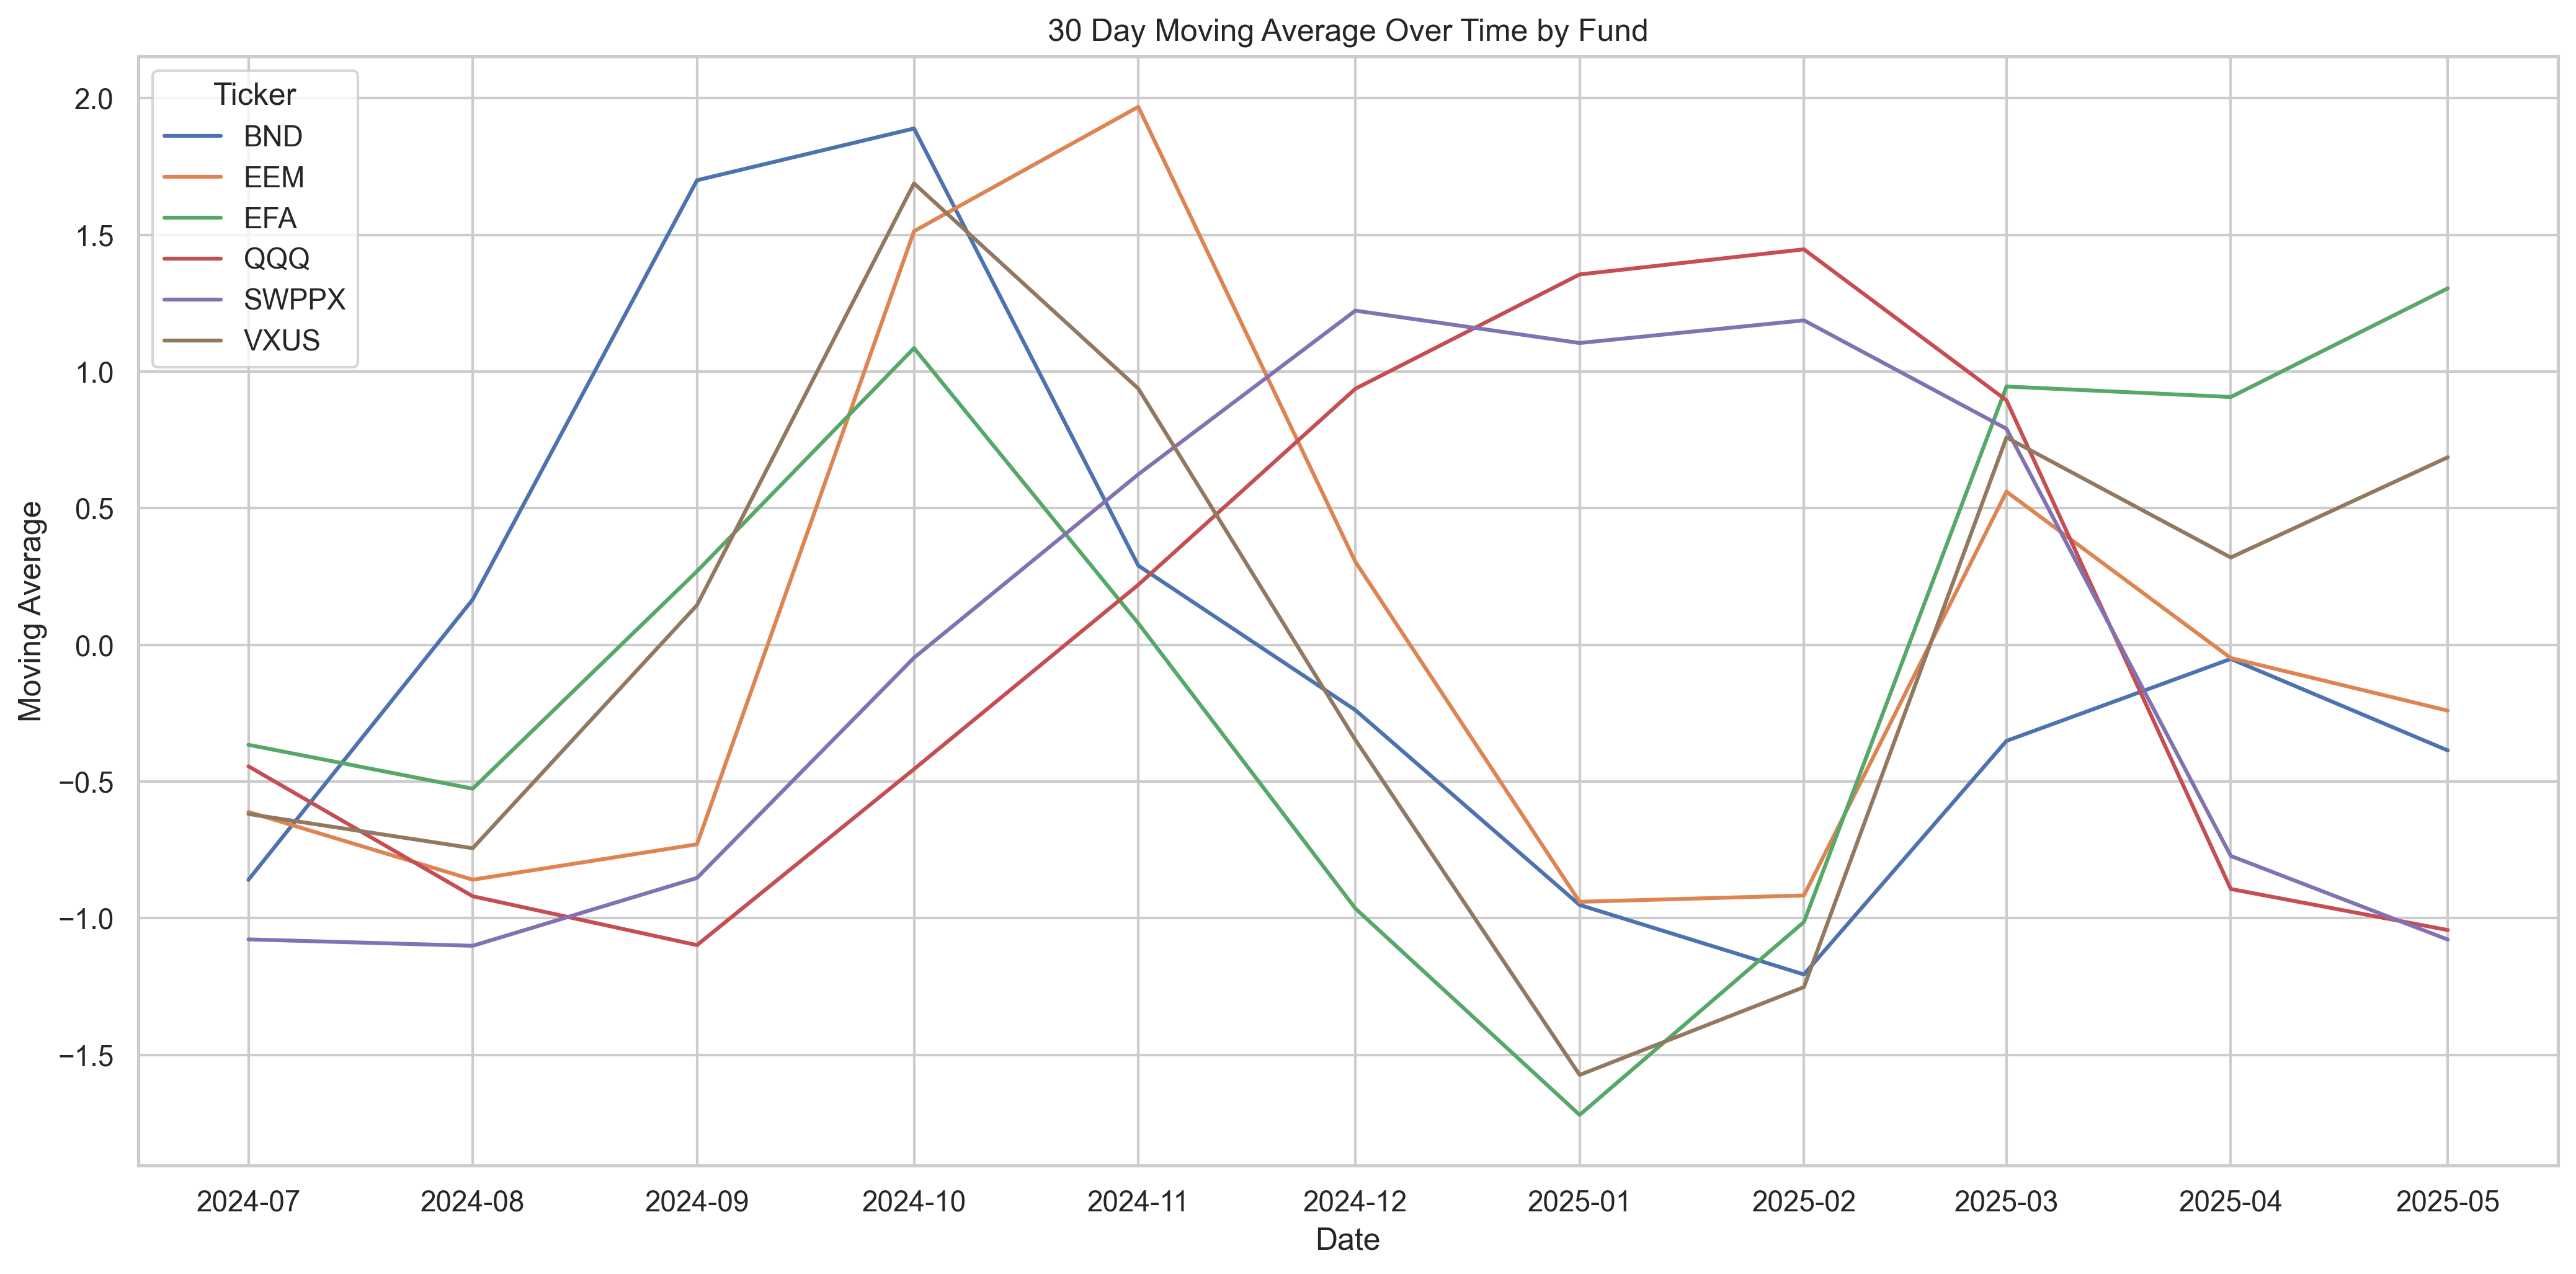
\includegraphics[width=0.65\linewidth]{\imgpath/MA_30.png} 
    \caption{30 Day Moving Average}
    \label{fig:MA_30}
\end{figure}

\subsection{Volatility over time}
The next graph will vizualize the volatility of the funds. This will also serve as a measure to see how suceptible the funds are to downturns or upturns in the market.

\begin{figure}[h]
    \centering
    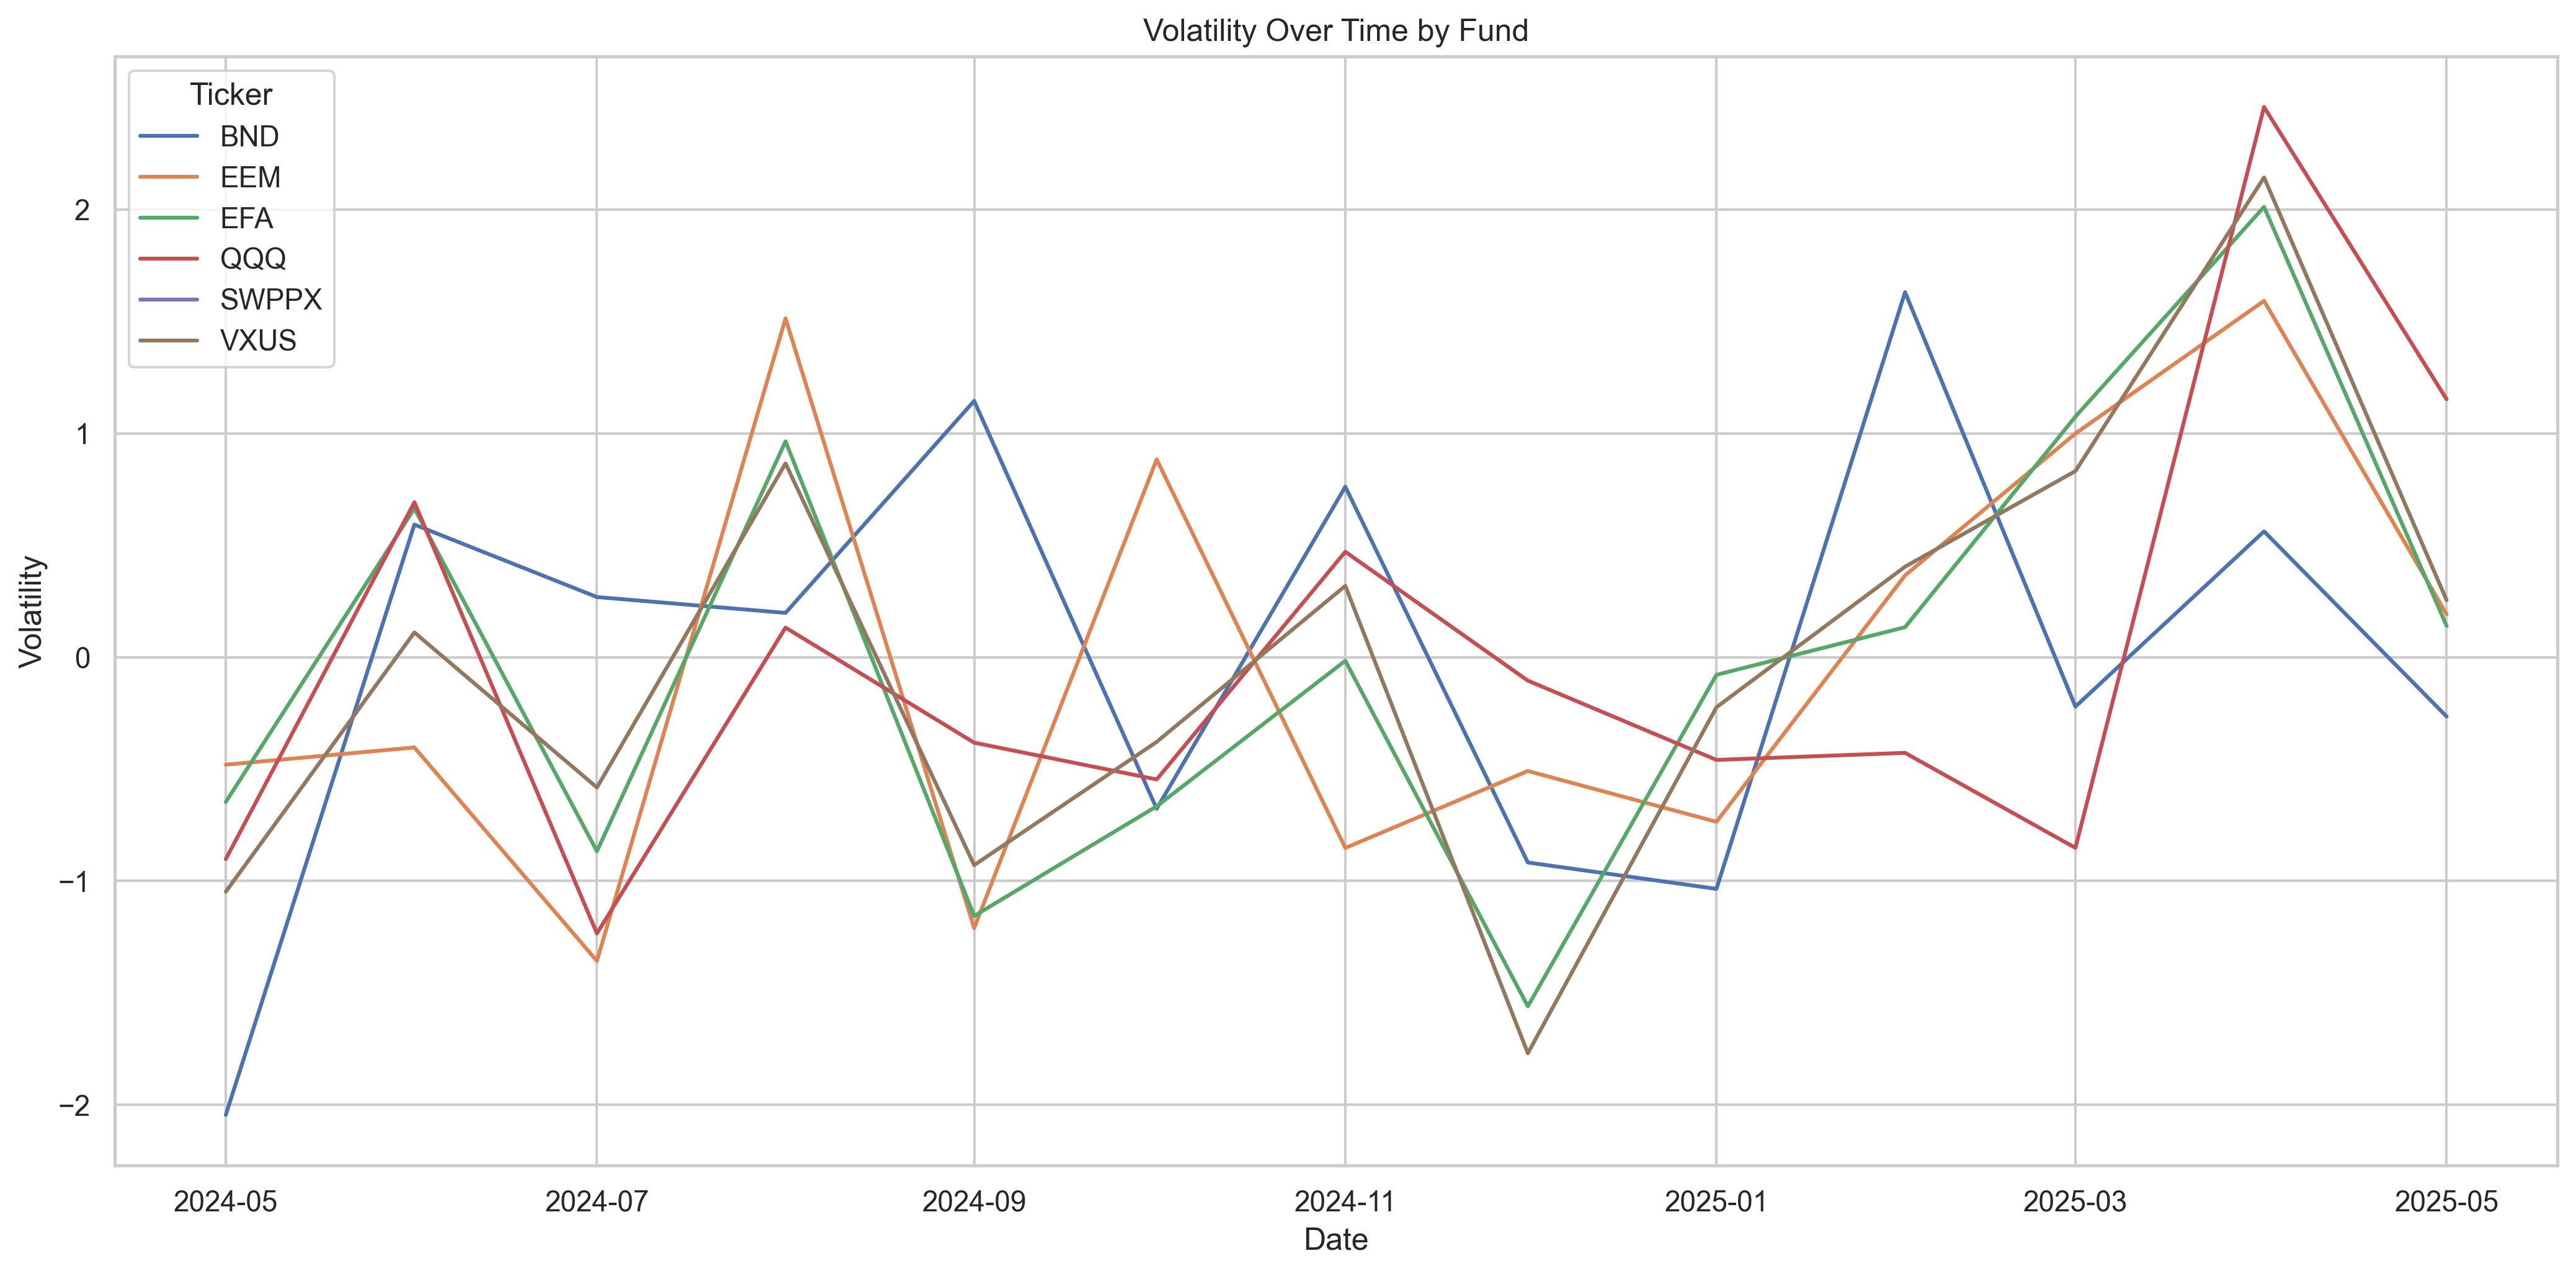
\includegraphics[width=0.65\linewidth]{\imgpath/Volatility.png} 
    \caption{Volatility}
    \label{fig:Volatility}
\end{figure}

\newpage

\subsection{Average Daily Returns}
While daily returns are not as useful a figure to focus on for establishing long-term trends, looking at how they averaged out each month could be a useful statistic regardless. This might provide more insight for short-term investors.

\begin{figure}[h]
    \centering
    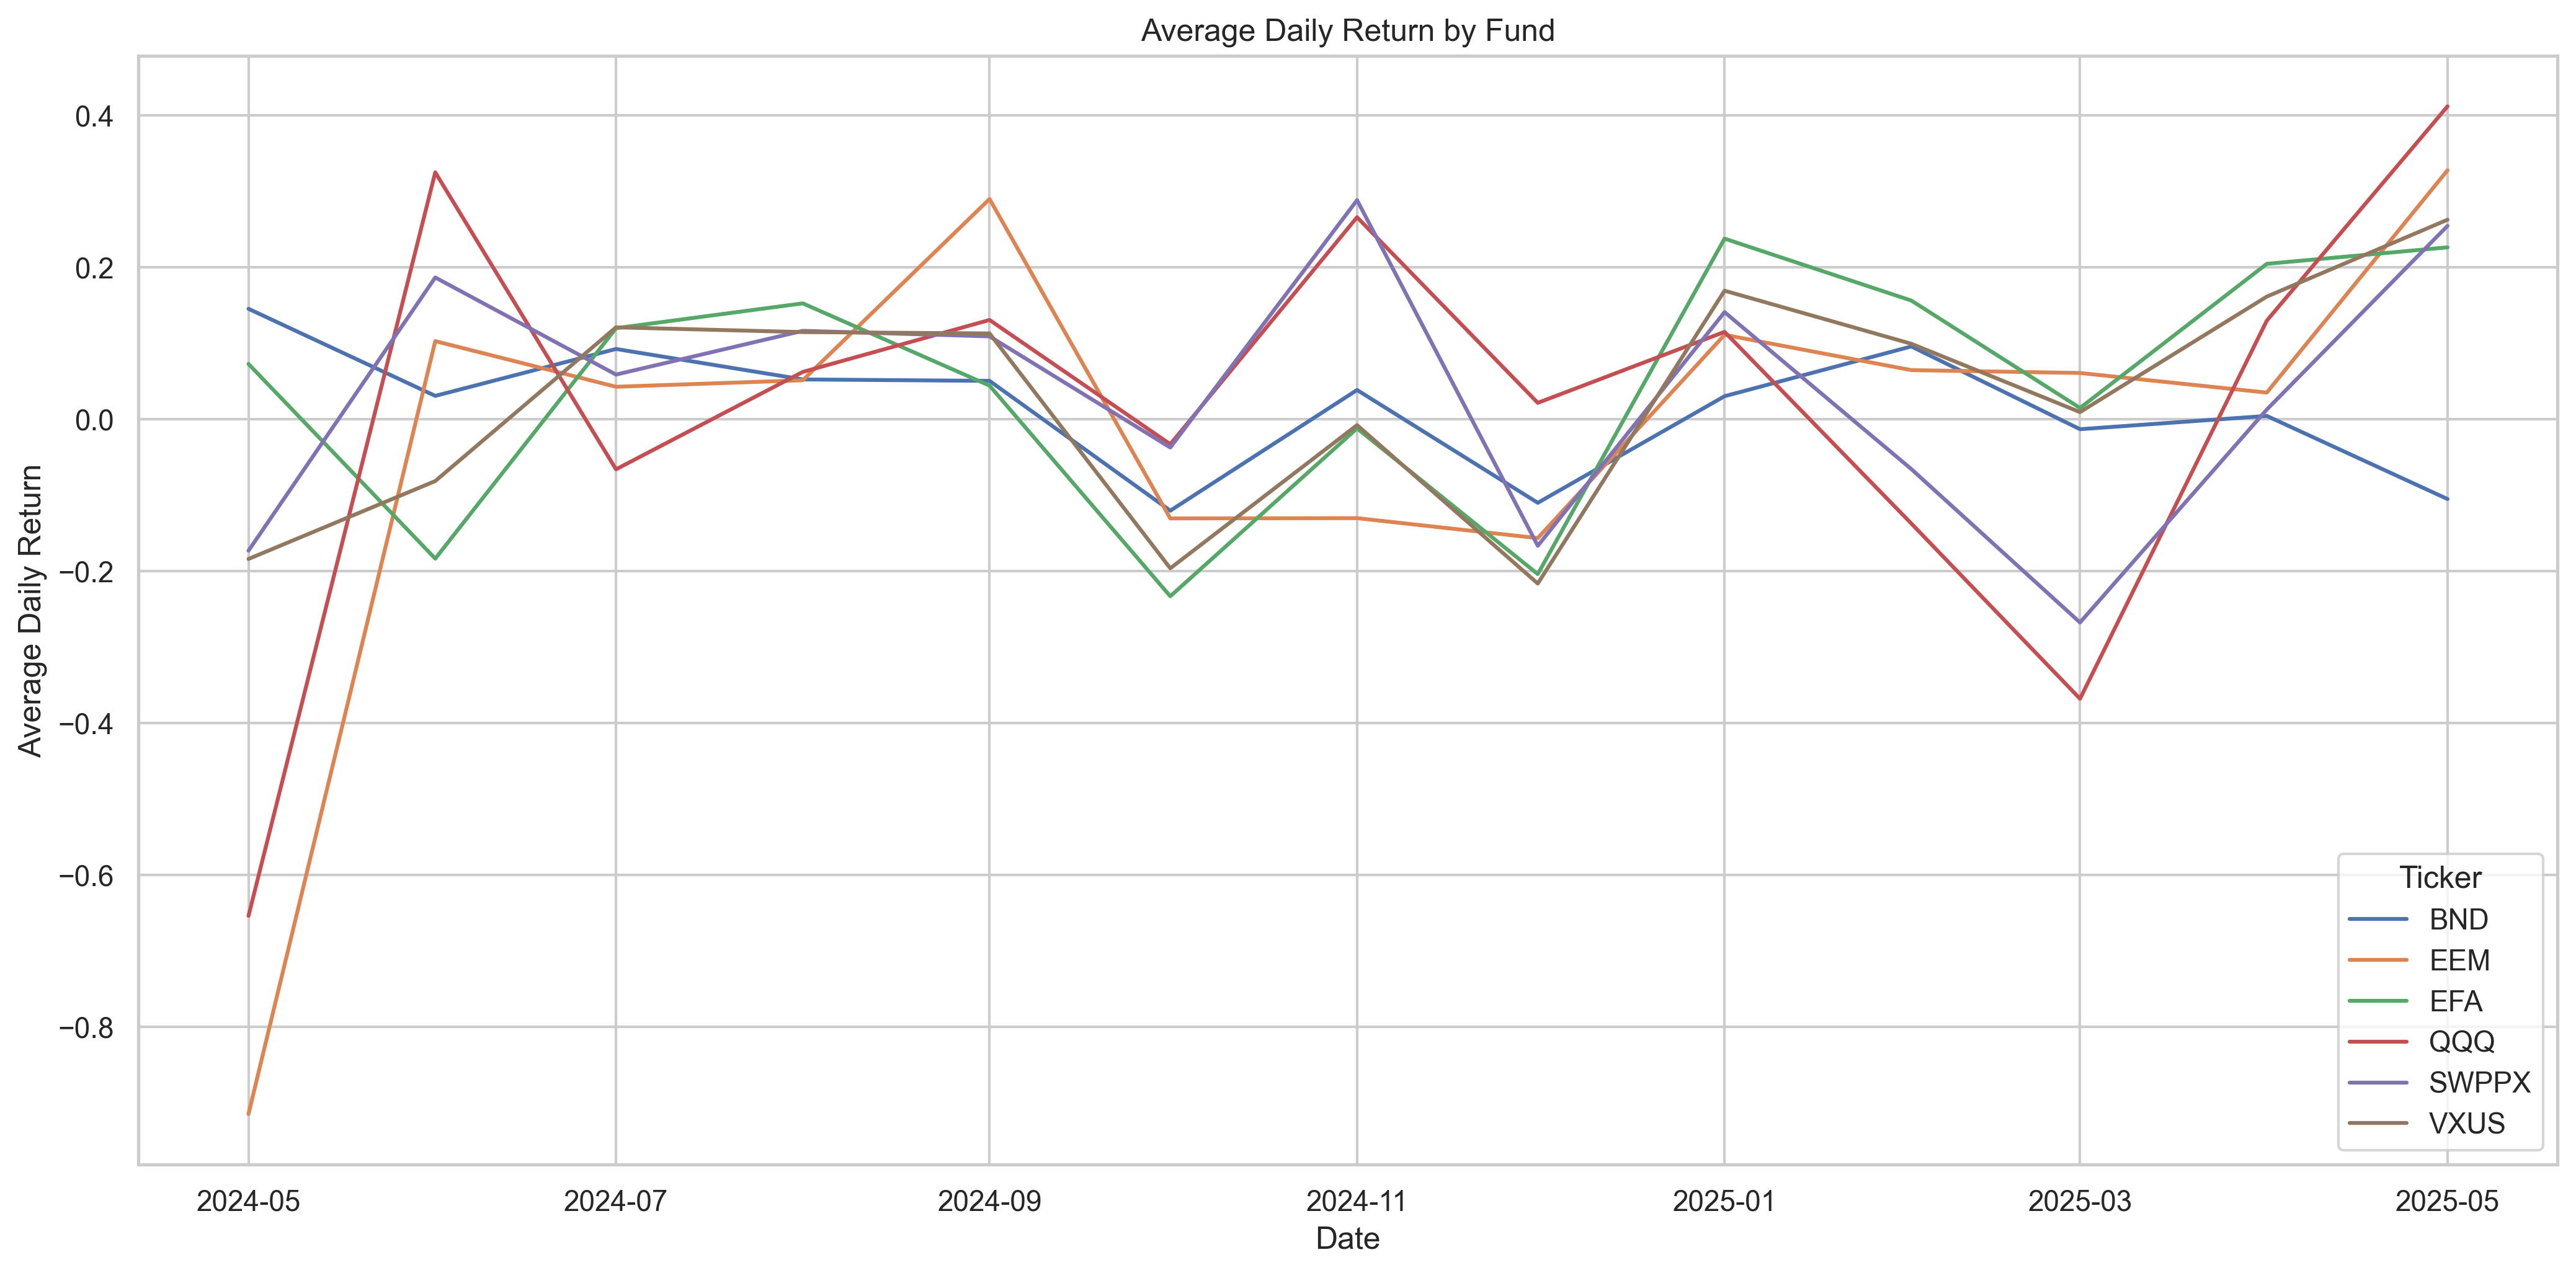
\includegraphics[width=0.65\linewidth]{\imgpath/Daily_Return.png} 
    \caption{Average Daily Return}
    \label{fig:Daily Return}
\end{figure}

\section{SQL Upload (03.00.SQL\_Upload.ipynb)}
This script connects to a PostgreSQL database using SQLAlchemy. It performs the following tasks:
\begin{itemize}
\item Reads the grouped weekly data CSV
\item Adds a Report\_Date column with the upload timestamp
\item Loads existing ticker and week ranges from the database
\item Deduplicates using a left join and filters new rows
\item Appends only new data to the stock\_prices\_weekly\_upd} table
\end{itemize}

\section{Fetch\_and\_Store.py}

This script serves as the Pipeline for the project. Essentially, it containerizes the processes in the (01.00.Data\_Cleaning.ipynb) and (03.00.SQL\_Upload.ipynb) scripts into a singular function called fetch\_and\_store. It performs the process of transforming the data then loading it to a postgres SQL project prepared specficially for the project. This makes it easier to implement the pipeline later on into an orchestrated deployment such as Airflow to automate the weekly upload of Data into the SQL server. This operation will of course be useful to any business that works with large volumes of data on a frequent basis.


\end{document}


